Die Topologie entspricht der vorgestellten Topologie der Infrastruktur (siehe Sektion \ref{sec: infra topologie}). Zusätzlich wird ein Back End in Form eines Servers benötigt, um den autonomen Verleih zu steuern. Die Abb. \ref{fig: impl topo} zeigt die Topologie der Implementierung.
\begin{figure}[H]
    \centering
    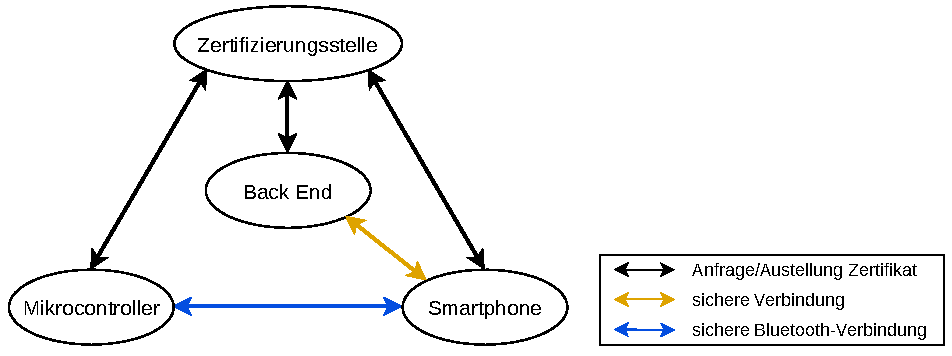
\includegraphics[width=1\textwidth]{graphics/impl_topologie.pdf}
    \caption[Topologie der Implementierung]{Topologie der Implementierung}
    \label{fig: impl topo}
\end{figure}
Bevor ein Ausleihprozess stattfinden kann, müssen Back End, Mikrocontroller und Smartphone jeweils über ein von der Zertifizierungsstelle ausgestelltes Zertifikat verfügen. Jeder Partei außer der Zertifizierungsstelle sollte periodisch (z.B. jährlich) ein Zertifikat ausgestellt werden.